% Defense 3 --- full report, single column, typeset directly in LaTeX.
% Build:  tectonic -X compile REPORT.tex   (or: tectonic REPORT.tex)
% Figures come from figures/out/*.pdf, each regenerated by figures/src/*.py.
\documentclass[10pt,a4paper,oneside]{article}

\usepackage[T1]{fontenc}
\usepackage[utf8]{inputenc}
\usepackage{times}
\usepackage[margin=1.05in,bottom=1.15in]{geometry}
\usepackage{amsmath,amssymb}
\usepackage{graphicx}
\usepackage{booktabs}
\usepackage{array}
\usepackage{longtable}
\usepackage{caption}
\usepackage{enumitem}
\usepackage{fancyhdr}
\usepackage{xcolor}
\usepackage{framed}
\usepackage{titlesec}
\usepackage[hidelinks]{hyperref}

\captionsetup{font=small,labelfont=bf,width=0.95\textwidth}
\setlength{\parskip}{0.45em}
\setlength{\parindent}{0pt}
\renewcommand{\arraystretch}{1.15}
\definecolor{keyc}{HTML}{1F5C99}
\definecolor{warnc}{HTML}{B03A2E}
\definecolor{shadecolor}{gray}{0.94}

\titleformat{\section}{\normalfont\large\bfseries\color{keyc}}{\thesection}{0.7em}{}
\titleformat{\subsection}{\normalfont\normalsize\bfseries}{\thesubsection}{0.6em}{}
\titlespacing*{\section}{0pt}{1.5em}{0.5em}
\titlespacing*{\subsection}{0pt}{1.1em}{0.35em}

\pagestyle{fancy}\fancyhf{}
\fancyhead[L]{\small\itshape Defense 3: a predetermined ACK delay for DNP3}
\fancyhead[R]{\small\thepage}
\renewcommand{\headrulewidth}{0.4pt}

% a boxed "the point is this" callout
\newenvironment{keybox}{\begin{snugshade}\noindent\ignorespaces}{\end{snugshade}}
\newcommand{\num}[1]{\mbox{#1}}
\newcommand{\code}[1]{\texttt{\small #1}}
\setlength{\emergencystretch}{3.5em}
\sloppy

\begin{document}

\begin{center}
{\LARGE\bfseries Defense 3: a predetermined acknowledgement delay\par}
\vspace{0.35em}
{\large\bfseries for DNP3, built in the data plane of a programmable switch\par}
\vspace{1.0em}
{\normalsize Validated on an Intel Tofino-1 against a physical SEL-751 protection relay\par}
\vspace{0.5em}
{\small 30 July 2026 \quad$\cdot$\quad 480 physical transactions \quad$\cdot$\quad
 \code{research/case-a-defense3-fixed-ack-delay}\par}
\end{center}

\vspace{0.8em}

\begin{keybox}
\textbf{How to read this document.} It starts with the physical world --- a relay in a
substation and someone watching the wire --- and narrows, step by step, to nanosecond
measurements inside a switch chip. Nothing is assumed: every term is defined where it
first matters, every formula is derived, and every number is either measured in this work
or marked as inherited. The verdict is stated early and then earned: \emph{the timing
fingerprint this defense targets is genuinely destroyed, and the defense that destroys it
is trivially visible to the same observer.} Both halves of that sentence are load-bearing.
\end{keybox}

\vspace{0.4em}
{\small\tableofcontents}
\clearpage

%======================================================================
\section{The setting, in plain terms}

An electrical substation contains \textbf{protection relays}: devices that watch the
current and voltage on a power line and open a breaker when something goes wrong. A
control centre talks to them over a network using an industrial protocol called
\textbf{DNP3}. A typical exchange is monotonous. The control centre asks ``what is your
status?''; the relay answers with a list of measurements. This repeats every second or so,
indefinitely.

Someone who can see that traffic --- a \emph{passive} observer, who cannot inject or alter
anything --- would like to know \textbf{what equipment is installed}. Knowing that a
particular cabinet holds an SEL-751 rather than some other relay tells them which
vulnerabilities to try, which firmware to study, and what the substation protects. In
security terms this is \textbf{reconnaissance}: the step before an attack.

Encryption does not solve it, for two reasons. First, a great deal of installed DNP3 is
unencrypted. Second and more fundamentally, \textbf{encryption hides what messages say,
not when they are sent}. If a device always takes about three milliseconds to think before
answering, that three milliseconds is visible whether or not the answer is encrypted.
Timing is a side channel, and a side channel is not closed by a cipher.

This work closes one specific timing side channel, in the network, without touching the
relay and without modifying a single byte of any packet.

\begin{figure}[t]
\centering

\includegraphics[width=4.35in]{figures/out/report/fig8_topology.pdf}
\caption{Where the switch sits. The relay and the master are both untouched software; the
switch between them runs the defense. Measurement is taken at the same point the
eavesdropper is assumed to observe, so every number in this report is a number the
attacker could obtain. Port numbers, front-panel positions and link speeds were read out
of the live switch configuration, not taken from a configuration file --- see
\S\ref{sec:physical}.}
\label{fig:topology}
\end{figure}

%======================================================================
\section{The vocabulary, defined once}

\begin{description}[leftmargin=1.4em,style=nextline,itemsep=0.35em]
\item[DNP3] The application protocol. For our purposes it runs over TCP, and a
  \emph{poll} is one request/response pair.
\item[A Class-0 READ] The commonest DNP3 request: ``send me your current static data''. It
  is \emph{read-only}. Nothing in this project ever sent a command that could change the
  relay's state; see \S\ref{sec:claims}.
\item[TCP acknowledgement (ACK)] TCP is the transport underneath DNP3. When a machine
  receives data, it sends back a tiny empty packet meaning ``got it''. That is an ACK. It
  is produced by the operating system's network stack, almost immediately, and carries no
  application data.
\item[Separate-ACK versus combined-ACK] When a relay receives a READ, two things must
  happen: TCP must acknowledge the bytes, and the application must compute an answer. Some
  devices send the ACK at once and the answer later --- \emph{two packets}, a
  \textbf{separate-ACK} device. Others wait and put both in one packet ---
  \textbf{combined-ACK}. This distinction is the whole ballgame.
\item[Case A / Case B] \textbf{Case A} is a separate-ACK device. The SEL-751 is one. Two
  packets means a measurable gap between them, and that gap is the target of this work.
  \textbf{Case B} is a combined-ACK device: one packet, no gap, nothing to hide. Case B is
  out of scope.
\item[CLRT --- Cross-Layer Response Time] The gap, on a separate-ACK device, between the
  transport acknowledgement and the application's answer. The name says what it is: an
  interval measured \emph{across} two layers.
\item[Tofino] A programmable switch chip. You write a program stating what the switch does
  to each packet; the language is \textbf{P4}. A Tofino is not a computer. It has no
  loops, no waiting, and a fixed budget of processing \emph{stages} through which every
  packet marches in lockstep. Everything in \S\ref{sec:mechanism} follows from those
  constraints.
\item[$D$] The one parameter of this defense: how long to hold the ACK back.
\end{description}

Formally, for one transaction, with $t_{\mathrm{READ}}$, $t_{\mathrm{ACK}}$ and
$t_{\mathrm{RESP}}$ the instants at which the observer sees the three packets:
\begin{equation}
\mathrm{CLRT} \;=\; t_{\mathrm{RESP}} - t_{\mathrm{ACK}},
\qquad
a \;=\; t_{\mathrm{ACK}} - t_{\mathrm{READ}},
\qquad
\text{total} \;=\; a + \mathrm{CLRT}.
\label{eq:defs}
\end{equation}
Throughout, $a$ is the relay's own acknowledgement latency and $c=\mathrm{CLRT}$ is the
quantity we are trying to hide. Keeping these three symbols straight is the whole of
\S\ref{sec:campaign}: a defense can shrink $c$ and yet leave the information intact
somewhere else in \eqref{eq:defs}.

%======================================================================
\section{The leak: why CLRT identifies a device}

When a relay receives a READ, its TCP stack acknowledges the bytes within a fraction of a
millisecond: cheap, mechanical work done by the network stack. Then the application
firmware wakes up, gathers measurements, formats a DNP3 response and sends it. How long
that second step takes depends on the relay's processor, its firmware, its scheduler and
how much data it must format --- in other words, \textbf{on what the device is}. Different
models differ. That is what makes CLRT a fingerprint.

The prior work that established this (Formby et al.) treats CLRT as a \emph{physical
property of the device} and uses it to identify equipment on a network. So the defensive
objective this project inherited is exactly: \textbf{make the observed CLRT stop revealing
the device}. That is the objective this report grades the defense against; grading it
against a broader one (``make the device unidentifiable'') is a different and much harder
question, treated honestly in \S\ref{sec:claims}.

Measured on the real SEL-751 with no defense running, 80 polls:

\begin{center}
\begin{tabular}{lr}
\toprule
\textbf{quantity} & \textbf{value} \\
\midrule
CLRT median & \num{2.828} ms \\
CLRT standard deviation & \textbf{\num{2.854} ms} \\
CLRT 95th percentile & \num{12.222} ms \\
CLRT maximum & \num{13.175} ms \\
\bottomrule
\end{tabular}
\end{center}

\textbf{The spread is the information.} A device whose CLRT is usually about \num{2.8} ms
with excursions to \num{13} ms looks different from one that is always at \num{0.4} ms.
The \emph{standard deviation} is the number to follow through this whole report, because a
defense that leaves the spread intact has hidden nothing, however much it moves the
median.

%======================================================================
\section{Three possible defenses, and the arithmetic that selects one}

Given a two-packet exchange and a switch in the middle, there are exactly three things the
switch can do to the gap.

\begin{description}[leftmargin=1.4em,style=nextline,itemsep=0.4em]
\item[Defense 1 --- hold the ACK until the response arrives, then release both.]
  The gap collapses to nearly zero. Already built in this project. Its flaw is structural:
  the switch releases the ACK \emph{because} the response arrived, so the ACK's timing now
  depends on the response. The interval $t_{\mathrm{READ}}\to t_{\mathrm{ACK}}$ becomes
  $a+c$, and $c$ is still there --- moved, not removed.
\item[Defense 2 --- forward the ACK at once, hold the RESPONSE to a fixed deadline $G$.]
  Also already built, and proven on this hardware against this relay. The observed CLRT
  becomes $G$, a constant. Its cost is latency: the answer is genuinely late by up to $G$.
\item[Defense 3 --- this work.] Forward nothing on demand. Hold the ACK to a fixed,
  \emph{predetermined} instant $t_{\mathrm{ACK}}+D$, chosen before the response is known
  and released independently of it. The response, if it arrives during the hold, queues
  \emph{behind} the ACK and leaves just after it.
\end{description}

The case for Defense 3 is arithmetic, not intuition. Writing $\delta$ for the small floor
left by the release machinery:

\begin{center}
\begin{tabular}{lccc}
\toprule
\textbf{defense} & \textbf{observer sees READ$\to$ACK} & \textbf{observer sees CLRT}
& \textbf{is $c$ visible?} \\
\midrule
none       & $a$     & $c$                        & \textbf{yes, directly} \\
Defense 1  & $a+c$   & ${\approx}\,0$             & \textbf{yes --- inside READ$\to$ACK} \\
Defense 2  & $a$     & $G$                        & no \\
Defense 3  & $a+D$   & $\max(c-D,\;\delta)$       & \textbf{no, when $D>c$} \\
\bottomrule
\end{tabular}
\end{center}

The last row is the point. Because the release instant is fixed \emph{in advance} and does
not depend on the response, $c$ appears in \textbf{neither} observable, provided
$D$ exceeds $c$:

\begin{equation}
\mathrm{CLRT}_{\text{out}} \;=\; \max\!\left(c - D,\; \delta\right),
\qquad
(t_{\mathrm{READ}}\!\to\! t_{\mathrm{ACK}})_{\text{out}} \;=\; a + D .
\label{eq:core}
\end{equation}

\begin{keybox}
\textbf{Consequence that drove the whole evaluation.} The right value of $D$ is not ``the
average CLRT''. Equation~\eqref{eq:core} conceals a transaction only when $D>c$, so
\textbf{only transactions faster than $D$ are hidden}. A $D$ set at the median hides about
half of them. This is why \S\ref{sec:campaign} sweeps $D$ instead of picking one.
\end{keybox}

Figure~\ref{fig:timelines} draws all four situations on one axis, with the measured
medians ($a=\num{0.45}$ ms, $c=\num{2.85}$ ms) so the geometry is to scale.

\begin{figure}[t]
\centering

\includegraphics[width=4.35in]{figures/out/report/fig4_timelines.pdf}
\caption{The same exchange with no defense and under each of the three defenses, to scale
with the measured medians. The orange span in each row is the interval that carries the
secret. Under Defense 1 the secret has simply moved from the CLRT into READ$\to$ACK. Under
Defense 3 neither interval contains $c$, provided $D>c$. ACK and RESPONSE are drawn in two
lanes per row because under Defenses 1 and 3 they leave within microseconds of one another
and would otherwise coincide. Source: \code{figures/src/fig4\_timelines.py}.}
\label{fig:timelines}
\end{figure}

%======================================================================
\section{How to delay a packet inside a chip that has no timers}
\label{sec:mechanism}

This is the hardest idea in the project and every later number depends on it.

A Tofino processes a packet through a fixed pipeline and sends it out. \textbf{There is no
instruction meaning ``hold this packet for two milliseconds''.} There is no timer you can
attach to a packet, no sleep, no programmable delay queue with a deadline. Packets go in
and come out.

What the chip does have is a \textbf{traffic manager} with queues and \textbf{strict
priority}. If queue~7 is strict-priority over queue~1, then for as long as queue~7 holds
anything at all, queue~1 is not served. That is the entire lever, and the mechanism is
built from it:

\begin{enumerate}[leftmargin=1.5em,itemsep=0.25em]
\item Put the ACK to be delayed into \textbf{$Q_{\mathrm{HOLD}}$} (queue 1, low priority)
  on an internal loopback port.
\item Fill \textbf{$Q_{\mathrm{BLOCK}}$} (queue 7, strict high priority) with dummy
  packets --- \textbf{blocker tokens} --- so $Q_{\mathrm{HOLD}}$ is starved and the ACK
  cannot leave.
\item Have each token, when it is served, read the clock, decide whether the deadline has
  passed, and if not \textbf{send itself around the loop again}. A recirculating token
  keeps $Q_{\mathrm{BLOCK}}$ non-empty.
\item Once the deadline passes, every token stops recirculating and is dropped.
  $Q_{\mathrm{BLOCK}}$ empties, $Q_{\mathrm{HOLD}}$ is served, and the ACK leaves.
\end{enumerate}

The delay is therefore produced by \textbf{a self-sustaining crowd of dummy packets that
gets out of the way at the right moment}. Nothing waits; everything is a packet being
processed normally, over and over.

\begin{figure}[t]
\centering
\makebox[\textwidth][c]{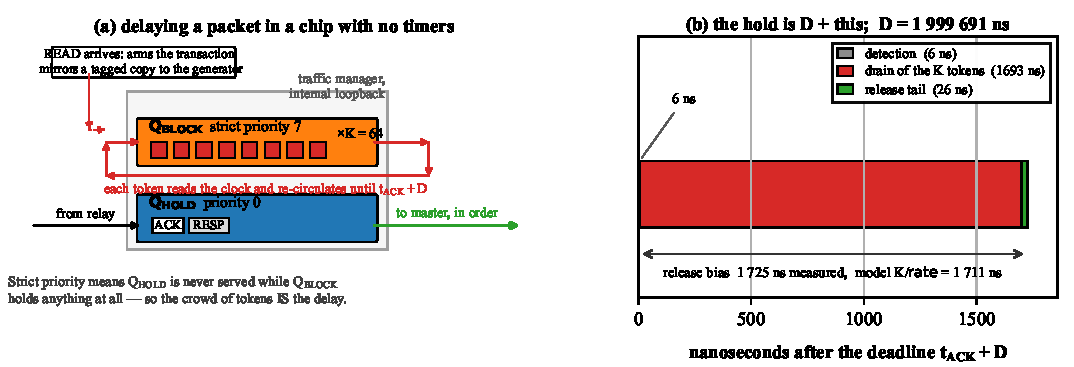
\includegraphics[width=7.16in]{figures/out/fig2_mechanism.pdf}}
\caption{\textbf{(a)} The construction. $Q_{\mathrm{BLOCK}}$ sits at strict priority 7 and
$Q_{\mathrm{HOLD}}$ at priority 0 on the same internal loopback port, so
$Q_{\mathrm{HOLD}}$ is never served while a single token remains. \textbf{(b)} What happens
\emph{after} the deadline, at nanosecond scale, measured on the physical relay. The hold is
$D$ plus these three terms, and $D$ itself is \num{1 999 691} ns --- three orders of
magnitude larger, which is why it cannot be drawn on the same axis.
Source: \code{figures/src/fig2\_mechanism.py}.}
\label{fig:mechanism}
\end{figure}

Three consequences matter.

\textbf{Why 64 tokens and not one?} A single token leaves gaps. After it is served it takes
a fraction of a microsecond to come back around, and in that window $Q_{\mathrm{BLOCK}}$ is
empty and the ACK escapes. Enough tokens must be in flight that the queue is
\emph{never} momentarily empty. $K=64$ was established as sufficient by earlier work in
this project, and every measurement here confirms it. It is \emph{not} claimed to be
minimal.

\textbf{Where do the 64 tokens come from?} The switch makes them itself. Tofino has a
\textbf{packet generator} that can be triggered by a pattern in a recirculated packet. When
a READ arrives and arms a transaction, the switch mirrors a small tagged copy of it to the
generator's port; the generator recognises the tag and emits 64 tokens. No external host is
involved --- which matters, because a defense that needs a server feeding it packets is not
a defense.

\textbf{What if something goes wrong?} Each token carries a \textbf{budget}: a maximum
number of loops. If the deadline somehow never arrives, tokens exhaust their budget and
stop anyway. This is the \textbf{fail-open} path --- the defense gives up and lets the
packet through rather than holding it forever and breaking the TCP connection.
\S\ref{sec:arith} gives the arithmetic that sets the budget.

%======================================================================
\section{The arithmetic}
\label{sec:arith}

Four numbers govern the mechanism. All are measured or derived; none are guessed.

\subsection{The deadline, and why \texorpdfstring{$D$}{D} is quantized}

The switch stores the deadline as a 32-bit word. Its low byte is reserved as an
armed/not-armed flag, so the time itself lives in the upper 24 bits, counted in units of
\num{256} nanoseconds --- one \emph{tick}. To hold for $D$ milliseconds:

\begin{equation}
\text{ticks} = \operatorname{round}\!\left(\frac{D\times 10^{6}}{256}\right),
\qquad
\text{word} = \text{ticks} \ll 8 .
\label{eq:ticks}
\end{equation}

The left shift puts a zero in the low byte so that the armed flag survives the later
addition. For $D=2$ ms:
\[
\text{ticks} = \operatorname{round}(2\,000\,000/256) = \num{7 812},
\qquad
\text{word} = \num{7 812}\ll 8 = \num{1 999 872}\ \text{ns},
\]
so $D_{\text{realized}} = \num{1.999872}$ ms and the shortfall is \num{128} ns.
\textbf{Every ``$D=2$ ms'' in this report means \num{1 999 872} ns.} That is quantization,
not a defect. $D$ is clamped at 40 ms, above which a hold would start to overlap the next
poll.

\subsection{The release bias: why the hold is longer than \texorpdfstring{$D$}{D}}

When the deadline passes, the tokens do not vanish together. Each one only learns of it the
next time it is \emph{served}. Draining $K$ tokens out of the queue at the loop's packet
rate takes

\begin{equation}
\tau \;=\; \frac{K}{r_{\mathrm{dp8}}}
      \;=\; \frac{64}{37.4\times 10^{6}\ \mathrm{pps}}
      \;=\; \num{1 711}\ \mathrm{ns},
\label{eq:tau}
\end{equation}

where \num{37.4} million packets per second is the \emph{measured} rate of the
25\,Gbit/s internal loopback for the small frames involved. So the ACK is released not at
the deadline but at approximately $\text{deadline}+\tau$.

This matters for honest measurement. Score the hold against $D$ and you see a systematic
$+\num{1 711}$ ns error on \emph{every} transaction, and you will be tempted to call it
jitter. The correct target is $D+\tau$, and every deadline number in this report is given
both ways: raw against $D$, and corrected against $D+\tau$.

\textbf{And $\tau$ was verified independently, which is the part that matters.} Originally
$\tau$ was a model whose only evidence was the residual it removed --- circular reasoning.
Instrumentation was added to timestamp the \emph{first} and \emph{last} token
terminations, so the drain could be measured directly:
\[
\text{predicted } \tau = \num{1 711}\ \text{ns}
\qquad
\text{measured drain} = \num{1 692}\text{--}\num{1 696}\ \text{ns}
\qquad
\text{agreement } 1.1\,\% .
\]

The full decomposition of one hold, from the synthetic gate, with each term measured
separately and nothing inferred:

\begin{equation}
\underbrace{\num{2 001 505}}_{\text{hold}}
=
\underbrace{\num{1 999 763}}_{D,\ \text{tick-quantized}}
+
\underbrace{\num{1 692}}_{\text{drain}}
+
\underbrace{27}_{\text{release tail}}
+
\underbrace{23}_{\text{detection}}
\quad \text{ns.}
\label{eq:decomp}
\end{equation}

\subsection{The fail-open horizon}

Each token may loop at most $B$ times. With $K$ tokens sharing the loop, the wall-clock
time before the last one gives up is

\begin{equation}
H \;=\; \frac{B\,K}{r_{\mathrm{dp8}}} \;=\; B\,\tau
  \;=\; \num{18 000}\times\num{1 711}\ \mathrm{ns} \;=\; \num{30.802}\ \mathrm{ms}.
\label{eq:horizon}
\end{equation}

$H$ has to sit inside a window. Too small and it fires during a legitimate hold, silently
turning a $D$-governed delay into a budget-governed one; too large and it approaches TCP's
retransmission timeout (measured at ${\approx}\,200$ ms), at which point the master gives
up and retransmits, which is a real fault. Both margins are clear:
\[
\frac{H}{\text{longest legitimate hold }(D=3\ \mathrm{ms})} = 8.8\times,
\qquad
\frac{200\ \mathrm{ms}}{H} = 6.5\times .
\]

An inherited comment in the code assumed \num{10}\,$\mu$s per loop, giving a horizon
\num{5.8}$\times$ wrong. It was replaced by \eqref{eq:horizon}, because a wrong model gives
a wrong answer the moment $K$, $B$ or the port speed changes. \textbf{Fail-open fired zero
times in every test in this report} --- the outcome you want: the safety net exists and was
never needed.

\subsection{The trigger chain}

How long after the READ does the reservoir actually exist? Measured over \textbf{100 clean
trials}, total spread \textbf{4 ns}:

\begin{center}
\begin{tabular}{lr}
\toprule
\textbf{step} & \textbf{time} \\
\midrule
READ arrives $\to$ tagged copy returns to the generator & \num{688} ns \\
generator recognises the pattern $\to$ first token admitted & \num{11} ns \\
all 64 tokens admitted (the burst itself) & \num{516} ns, ${\approx}\,8$ ns per token \\
\midrule
\textbf{READ $\to$ full 64-token reservoir} & \textbf{\num{1 215} ns} \\
\bottomrule
\end{tabular}
\end{center}

Compare that with the relay's own acknowledgement latency --- the earliest moment there is
anything to hold --- measured at \num{0.453} ms median, \num{0.400} ms minimum. The
reservoir is ready roughly \textbf{330 times sooner than it needs to be}
(Figure~\ref{fig:trigger}). There is no race, and the cold first trial after a program load
sits inside the warm distribution, so there is no warm-up cost either.

\begin{figure}[t]
\centering

\includegraphics[width=4.35in]{figures/out/report/fig6_trigger.pdf}
\caption{The trigger chain against the deadline it must beat, on a logarithmic axis because
the two live three orders of magnitude apart. The reservoir is complete \num{1 215} ns after
the READ; the earliest the relay's own ACK can arrive is \num{400 000} ns. The margin is
${\approx}\,330\times$, which is why the arming path never races the traffic it protects.
Source: \code{figures/src/fig6\_trigger.py}.}
\label{fig:trigger}
\end{figure}

%======================================================================
\section{The implementation, and four hardware traps}
\label{sec:traps}

The switch program is \code{p4/case\_a\_defense3\_fixed\_ack\_delay.p4}. Its shape is
simple: decide in the parser what each packet \emph{is}, resolve every remaining condition
in \emph{one} table lookup, then act. What is not simple is the hardware. Four separate
traps were found, and \textbf{the compiler accepted all four without complaint}.

\subsection{Trap one --- a large constant in stateful hardware silently does nothing}

The switch keeps a small amount of memory a packet can read \emph{and} modify as it passes:
a \textbf{register} with a tiny attached processor, the \textbf{stateful ALU} (SALU). One
register, \code{reg\_tag}, holds the ``which transaction is currently live'' marker.

The code said: \emph{if the marker says idle, write my transaction's identity into it}.
Idle was originally encoded as \code{0xFF}. On hardware, \textbf{the write never happened.}
The transaction never became live, so all 64 tokens were rejected and the relay's ACK was
refused. But the same tiny processor also \emph{returns} a value, and that path worked
perfectly --- so a counter reported ``a new transaction was armed'' while the register said
no transaction existed. That contradiction produced two wrong diagnoses before the compiled
assembly was read:

\begin{center}\small
\begin{tabular}{@{}ll@{}}
\code{sub hi, phv\_lo, lo}      & the RETURN value \quad---\quad worked \\
\code{equ lo, lo, -255}         & the PREDICATE \quad---\quad never true \\
\code{alu\_a cmplo, lo, phv\_lo} & the conditional write, therefore never executed \\
\end{tabular}
\end{center}

Changing idle from \code{0xFF} to \code{0x00} made the predicate \code{equ lo, lo} --- a
comparison against zero, needing no embedded constant --- and the write began to commit.
Tokens admitted went from \textbf{0 to 64}.

\textbf{A correction against ourselves, which is why a probe exists.} The obvious
explanation is ``255 is too wide for the instruction's constant field''.
\code{p4/probe\_salu\_immediate.p4} tests that by comparing thirteen registers against
$K \in \{1,2,7,8,15,16,63,64,127,128,192,254,255\}$. \textbf{The compiler emits
\code{equ lo, lo, -K} for every one of them, identically, with no error and no warning.} So
the assembly \emph{cannot} distinguish a safe constant from an unsafe one, and the width
explanation is an inference consistent with the evidence, not a proof. The repair is
confirmed behaviourally on silicon; the mechanism is not.

\begin{keybox}
\textbf{The usable rule is structural, not an inspection:} never compare stateful state
against a large constant. Compare against zero, or against a value carried in the packet.
It is enforced by a test,
\code{analysis/test\_tag\_domain.py}, not by discipline. After
the repair, exactly \emph{one} constant comparison remains anywhere in the program ---
against 2 --- and that one is proven working on hardware.
\end{keybox}

\subsection{Trap two --- a sign test that is always false}

Later work needed ``is the top bit of this byte set?'', which is naturally written as ``is
this value negative''. Written the obvious way on an unsigned byte,
\code{if (v < 8w0)} compiles fine and emits \code{lss.u lo, lo}. But \code{lss.u} is an
\emph{unsigned} less-than-zero: it is never true. The compiler reported success. With an
explicit signed cast, \code{if ((int<8>)v < 8s0)} emits \code{lss.s lo, lo}, which is
correct.

Two silent miscompiles in the same small piece of hardware was enough to stop trusting
inspection, so \code{analysis/assert\_salu\_asm.py} now \textbf{fails the build} if the
compiled assembly for the load-bearing predicates contains \code{lss.u} or is missing the
expected instructions. It is mutation-checked: reverting the cast makes the compiler exit 0
while the assertion exits 1.

\subsection{Trap three --- four operations per register, and it is a hard error}

Adding a fifth way of touching \code{reg\_tag} produced
\code{error: too many RegisterActions attached to the Register; the target architecture
limits the number to 4}.

This forced a genuinely better design. One of the five was a plain read, used by the
blocker tokens --- and a read is just a modification that adds zero. So the read and the
``mark this transaction'' operation were merged into a single operation whose increment
arrives in the packet's metadata: \code{0x50} to mark, \code{0} for a plain read. Four
operations, nothing lost.

\subsection{Trap four --- the chip has two pipelines, and a timer fires in both}

An early synthetic test emitted three events and observed six. The chip has two pipelines,
and enabling a packet-generator application device-wide arms it in \emph{both}. A
pattern-triggered application is masked from this --- only one pipeline sees the trigger ---
but a timer-triggered one fires everywhere it is armed. Every generator write is now scoped
to one pipeline. From the same session: \code{pgrep -f bf\_switchd} over-counts (it returned
3 for one process); \code{pgrep -cx} is correct.

%======================================================================
\section{The state machine, and the bug that took two attempts}
\label{sec:fsm}

\subsection{What the state has to express}

One register byte, \code{reg\_tag}, must express three things at once:

\begin{center}
\begin{tabular}{ll>{\raggedright\arraybackslash}p{0.36\textwidth}}
\toprule
\textbf{meaning} & \textbf{encoding} & \textbf{how it is distinguished} \\
\midrule
no transaction in progress & \code{0x00} & the value zero \\
live, no response yet & \code{0xC0}--\code{0xCF} & \textbf{top bit set} \\
live, response already queued & \code{0x10}--\code{0x1F} & \textbf{top bit clear}, never zero \\
\bottomrule
\end{tabular}
\end{center}

The \code{0xC0}--\code{0xCF} range is not arbitrary. DNP3's application header byte for a
first-and-final, solicited, unconfirmed request is \code{0xC} in the top nibble and a 4-bit
sequence number in the bottom --- so \emph{the protocol hands us} a per-transaction identity
in exactly that range, and the parser accepts a READ only if its byte is in it. That is also
the proof that \textbf{no live identity can ever be zero}: there is no arithmetic on it
anywhere, the sequence advances inside the low nibble only, and the top nibble is pinned by
the parser's own acceptance test.

The third state is reached by \textbf{adding \code{0x50}}: $\code{0xC}n + \code{0x50} =
\code{0x1}n$. That is one hardware instruction; it is one-shot for free, because adding
\code{0x50} clears the top bit so applying it twice does nothing the second time; and it
\textbf{keeps the identity}, since the low nibble still says which transaction. It is a
state, not a flag. Figure~\ref{fig:fsm} draws the result.

\begin{figure}[t]
\centering

\includegraphics[width=4.35in]{figures/out/report/fig5_statemachine.pdf}
\caption{The transaction state machine: three disjoint domains inside one byte. The two
live states differ only in the top bit, so the switch separates them with a single signed
comparison against zero (\S\ref{sec:traps}). The white lines inside the live boxes are what
a circulating blocker token computes --- the identity it carries minus the value it finds.
Because the marking transition \emph{adds} a constant rather than overwriting, that
difference is \code{0x00} before marking and \code{0xB0} after, so one extra table entry
covers all sixteen identities and the reservoir survives the state change.
Source: \code{figures/src/fig5\_statemachine.py}.}
\label{fig:fsm}
\end{figure}

\subsection{The bug: a missing exit}

Gate 4 case C tested the obvious failure --- the relay acknowledges but never answers. The
result was clean on every count except one: \textbf{the transaction never ended.}
\code{reg\_tag} was left holding a live identity forever, and the \emph{next} poll was
therefore refused as a concurrent transaction: no reservoir, no hold, an unprotected
transaction.

The cause is a two-line proof. There were exactly two ways to end a transaction: the
released response ends it, and the fail-open budget ends it. With no response the first
cannot fire; and the tokens die on the \emph{deadline}, so they never reach their budget ---
the deadline \textbf{pre-empts} the second. Neither exit fires. The measured cost was
exactly \textbf{one} subsequent unprotected transaction, after which the system self-heals,
because that transaction's own response clears the stale identity on its way out.

\subsection{The repair that could not be built}

The natural fix is to record ``a response is pending for transaction $g$'' in a second
register, and on the ACK's release check whether it matches. It \textbf{does not compile}:
\emph{``Table placement cannot make any more progress\ldots{} dependency analysis has
found that no more tables are placeable.''}

The reason is structural, not incidental. The response path must read the identity register
\emph{before} writing the pending register; the ACK-release path needs the opposite order.
Register placement in this hardware is \textbf{static} --- each register lives in exactly one
pipeline stage --- so two registers with opposite orderings on two paths form a dependency
cycle, even though the two paths are mutually exclusive at run time. The condition that
separates them is invisible to placement.

\code{p4/probe\_retire\_dependency.p4} reduces this to the smallest reproduction: two
byte-sized registers, two paths, opposite orders, nothing else. \code{-DPROBE\_CYCLE}
reproduces the error verbatim; keeping the state \emph{inside} the existing register
(\code{-DPROBE\_ONE\_REG}) compiles in two stages. That is why the design is as it is.

\subsection{The repair that was built}

\begin{itemize}[leftmargin=1.4em,itemsep=0.2em]
\item when the first response of a transaction is admitted, add \code{0x50} (one-shot by
  construction);
\item on the ACK's release, \textbf{if the top bit is still set} --- nothing pending ---
  end the transaction immediately;
\item if the top bit is clear, a response is queued, so leave the transaction live and let
  that response end it, exactly as before.
\end{itemize}

One extra table entry was required. When the marker changes, the circulating tokens are
comparing themselves against a value that just moved. The difference a token computes is
$\text{carried identity} - \text{stored value}$, which for a marked tag is
$\code{0xC}n - (\code{0xC}n - \code{0xB0}) = \code{0xB0}$ for \emph{every one} of the
sixteen identities. So it is a single exact entry, not sixteen --- and if it were wrong the
failure would be immediate and loud: the tokens would read as foreign, the reservoir would
collapse before the deadline, and the counters would show it. \code{BLOCK\_TERM\_STALE} was
\textbf{0} in every subsequent test.

\textbf{A free bonus fell out of the encoding.} ``Response pending'' is a \emph{distinct
value}, not a flag, so every pre-existing test of the form ``live and nothing pending yet''
keeps its exact meaning --- and a duplicate response therefore misses the hold branch by
itself, with no new code. That is how \S\ref{sec:gates} handles duplicates.

\subsection{A defect that the repair itself introduced}

Moving ``idle'' to \code{0x00} collided it with a \emph{different} constant already meaning
``leave this register alone'' --- also \code{0x00}. Both transaction-ending paths write
``idle'' through the operation guarded by that constant, so \textbf{both silently became
no-ops}. Nothing had run yet; it was caught by an audit, not by a failure.

\begin{keybox}
\textbf{General lesson:} a fix that moves a sentinel value must enumerate every other
sentinel in the same field. The distinct-value constant was moved to \code{0x01}, which is
safe because the field only ever holds that constant, idle, or an identity in
\code{0xC0}--\code{0xCF}.
\end{keybox}

\subsection{The final state-transition table}

\begin{center}\small
\begin{tabular}{@{}>{\raggedright\arraybackslash}p{0.185\textwidth}>{\raggedright\arraybackslash}p{0.115\textwidth}>{\raggedright\arraybackslash}p{0.115\textwidth}>{\raggedright\arraybackslash}p{0.108\textwidth}>{\raggedright\arraybackslash}p{0.238\textwidth}@{}}
\toprule
\textbf{event} & \textbf{before} & \textbf{action} & \textbf{after} & \textbf{packet's fate} \\
\midrule
READ, nothing in progress & \code{0x00} & write identity & \code{0xC}$n$ & armed; mirror triggers 64 tokens \\
READ, one in progress & \code{0xC}$n$ or \code{0x1}$n$ & no write & unchanged & refused as concurrent, forwarded unprotected \\
token, fresh & \code{0xC}$n$ & read (increment 0) & unchanged & admitted to $Q_{\mathrm{BLOCK}}$ \\
token, difference \code{0x00} or \code{0xB0} & either live state & read only & unchanged & still ours, loops again \\
token, foreign identity & any & read only & unchanged & stale, dropped \\
\textbf{first response, in window} & \code{0xC}$n$ & \textbf{add \code{0x50}} & \textbf{\code{0x1}$n$} & queued in $Q_{\mathrm{HOLD}}$ \emph{behind} the ACK \\
\textbf{duplicate response} & \code{0x1}$n$ & nothing & \code{0x1}$n$ & \textbf{suppressed} \\
\textbf{ACK release, response pending} & \code{0x1}$n$ & nothing & \code{0x1}$n$ & forwarded; transaction stays live \\
\textbf{ACK release, nothing pending} & \code{0xC}$n$ & \textbf{write idle} & \textbf{\code{0x00}} & forwarded; \textbf{transaction ends here} \\
queued response released & \code{0x1}$n$ & write idle & \code{0x00} & forwarded; transaction ends here \\
response after the end & \code{0x00} & nothing & \code{0x00} & forwarded once, never held \\
tokens exhaust the budget & \code{0xC}$n$ & write idle & \code{0x00} & fail-open \\
\bottomrule
\end{tabular}
\end{center}

\code{analysis/test\_tag\_domain.py} checks this model \textbf{exhaustively rather than by
example}: all sixteen identities, all 240 ordered pairs of distinct identities, both
markers, every transition --- \textbf{\num{2 256} assertions, 0 failures}. It is
mutation-checked four ways (revert the idle marker $\to$ 10 failures; re-collide the
sentinels $\to$ 66; change the increment from \code{0x50} to \code{0x40} $\to$ 317; to
\code{0x00} $\to$ 195), because a test that cannot fail proves nothing.

%======================================================================
\section{Validation on synthetic traffic: gates 1 to 4}
\label{sec:gates}

Before touching the relay, the mechanism was exercised with packets the switch generated
itself. This is not a formality: it is the only way to test cases a real relay will not
produce on demand, such as a response that never comes.

\textbf{How the synthetic events are made, and a hardware law discovered doing it.} The
events (READ, ACK, RESPONSE) are emitted by the switch's own packet generator. The first
attempt put all three in one generator \emph{run}, spaced by a hardware gap. The reservoir
then stood \num{1 000 012} ns after the READ instead of \num{1 215} ns --- the ACK had
already escaped.

\begin{keybox}
\textbf{The packet generator will not start a triggered burst while another generator run is
in progress, and the wait equals the whole run's span --- including its idle gaps.}
Measured at four points: a 3-packet run with a 200\,$\mu$s gap delayed the burst by
400\,$\mu$s; with a 500\,$\mu$s gap, by 1\,000\,$\mu$s; two 1-packet runs with a
500\,$\mu$s inter-run gap, by 500\,$\mu$s; three with 200\,$\mu$s, by 400\,$\mu$s. In every
case the tagged copy was emitted on time (688 ns) and the delay was \emph{inside} the
generator. Reproduced to the nanosecond: \num{1 000 012} ns.
\end{keybox}

Two further attempts failed for reasons worth knowing: a pattern-triggered generator
application \emph{cannot label its own packets} (all three decoded as the same one, so the
roles collapsed), and two applications sharing one trigger are served events-first with no
control-plane way to order them. The working schedule uses \textbf{two timer applications}
--- one emits the READ alone, the other the ACK and RESPONSE --- \textbf{armed in a single
write}, so the software skew (measured at \num{1.15} ms with two separate writes) cannot
leak into the offset. The realised READ$\to$ACK offset came out \textbf{10 ns} from target.

\subsection{Gate 1 --- does it load, and is the hardware configured}

Both compilers agree exactly (9 stages, no drift); the program loads; strict priority is
confirmed as $7>0$; $K=64$ is confirmed; the fail-open horizon is confirmed as
\num{30.802} ms.

On the \emph{first} attempt this gate \textbf{aborted}, because the internal loopback port
was at 10\,Gbit/s instead of 25. That is not cosmetic: the token drain rate, and therefore
both $\tau$ and $H$, scale with it. The check that caught it is now permanent and blocking.

\subsection{Gate 2 --- one transaction, seventeen requirements}

\textbf{PASS, 17/17.} The headline is the decomposition already given in
\eqref{eq:decomp}, with reservoir standing \num{678} ns, READ$\to$ACK \num{500 010} ns,
ACK$\to$RESPONSE $+28$ ns (positive, so the order is right), and fail-open zero. Evidence:
\code{evidence/gate2/gate2\_20260729T231747Z/}, scored by
\code{analysis/analyze\_defense3.py}, whose self-test carries 17 negative controls proving
each requirement can actually fail.

\subsection{Gate 3 --- five consecutive transactions, no reset between them}

\textbf{PASS, 5/5, 18 requirements each.} The identity was \emph{advanced} each time
(\code{0xC0}$\to$\code{0xC4}), so a transaction that failed to end could not be mistaken for
one that did --- it would be refused as concurrent, exactly the signature described above.

\begin{center}
\begin{tabular}{lrrr}
\toprule
\textbf{quantity} & \textbf{min} & \textbf{max} & \textbf{spread} \\
\midrule
hold                & \num{2 001 427} & \num{2 001 586} & \textbf{\num{159} ns} \\
drain               & \num{1 691}     & \num{1 695}     & \textbf{4 ns} \\
release tail        & 26              & 28              & \textbf{2 ns} \\
reservoir standing  & \num{1 193}     & \num{1 195}     & \textbf{2 ns} \\
READ$\to$ACK        & \num{500 009}   & \num{500 011}   & \textbf{2 ns} \\
\bottomrule
\end{tabular}
\end{center}

\textbf{The first attempt at this gate failed on our own criterion, not on the defense.} The
rule demanded that two registers be zero between transactions. They were not --- they held
the previous transaction's deadline and identity --- but the architecture never promised they
would be: both are \emph{self-clearing by design} (the next READ overwrites the deadline
unconditionally; the response test is a \emph{difference}, so a new identity reads non-zero
with no reset). The replacement rule is \textbf{stricter}, not looser: it keeps ``the
transaction ended'' and adds a check the old rule could not even see --- that the inherited
value must not collide with the new identity, which would silently invert the early/late
classification.

\subsection{Gate 4A --- a response arriving just before the deadline}

\textbf{PASS 3/3}, with the response arriving \num{4 872} ns before the deadline. Shrinking
the margin from 1.5 ms to under 5\,$\mu$s changed nothing, which is the point of the case.

\subsection{Gate 4B --- a response arriving after the acknowledgement has gone}

\textbf{PASS 3/3}, response \num{500 128} ns late. It takes the normal forwarding path,
forwarded exactly once, never held, and cannot disturb a later transaction. This is a
\emph{deliberate behaviour change}: before the state-machine repair a late response was
briefly held; now the transaction has already ended, so it simply goes through. That is
better --- it costs one less internal loop.

\subsection{Gate 4C --- the relay never answers}

\textbf{PASS 3/3 after the repair}, and this is the case that produced \S\ref{sec:fsm}. The
ACK's release now ends the transaction, \code{reg\_tag} returns to idle, and --- the
requirement that matters --- \textbf{the very first following transaction is fully
protected}, three times out of three. Before the repair, that transaction was completely
unprotected.

\subsection{A duplicate response, and an invariant that was being violated}

If the relay retransmits its response while the first copy is still queued, what happens?
The first answer was ``the duplicate is forwarded'' --- and measurement showed that was
wrong. Across three repetitions the duplicate departed \num{1 001 449}, \num{1 001 341} and
\num{1 001 421} ns \emph{before} the held ACK.

\textbf{The duplicate overtook the very packet the defense exists to delay, by
\num{1.0014} ms}, because the forwarding path goes straight out while the ACK is still
queued. The gate had reported PASS: the rubric never tested ordering. It was found by adding
a timestamp and looking.

The repair --- the term for it is \textbf{current-transaction identity-matched response
retransmission suppression} --- drops such a copy while a response of that identity is
already pending, and counts it separately. ``Identity-matched'' means: same TCP sequence
position, same acknowledgement relationship, same learned session port, the same DNP3
solicited single-fragment framing, and the same transaction identity.

\textbf{It is deliberately not called byte-exact.} The response's length and payload bytes
are \emph{not stored anywhere}, so they are not compared. A retransmission carrying the same
sequence number but a \emph{different} length is the one case this cannot distinguish.
Storing the length would mean new permanent state, which the design does not have room for.
Enqueuing a second copy instead of dropping it was rejected because a queued response ends a
transaction unconditionally, so a second copy could end a \emph{later} one.

After the repair: \textbf{3/3} --- first response held and marking, duplicate suppressed,
nothing forwarded early, and the bypass timestamp never written at all. A second measurement
bug of ours was found the same way: the first version of that timestamp also fired on the
\emph{suppressed} copy, a packet that had been dropped and therefore departed nowhere.

\subsection{A stale response arriving during a live transaction}

The hardest isolation case. Transaction $N$ finishes, $N{+}1$ arms with its reservoir
standing and its deadline set, and then a response belonging to $N$ arrives.

Making this test honest required work, because \textbf{the identity a response carries is
its TCP sequence position}, and the ACK and the response are tested against the \emph{same}
register --- so one packet template cannot produce ``stale response, valid
acknowledgement''. A third generator application with its \emph{own} packet buffer and a
sequence number offset by \code{0x1000} was added, firing 800\,$\mu$s after the READ.

\textbf{PASS 3/3.} $N{+}1$'s identity unchanged, its deadline unchanged, its pending marker
unchanged (proven by the ACK still finding the marker set), its 64 tokens unchanged with
zero stale terminations, the stale copy not held and not suppressed --- correctly taking the
bypass path, because a \emph{different} identity must not be suppressed --- and $N{+}1$
ending cleanly on its own response.

\subsection{Resource cost of the whole thing}

\begin{center}
\begin{tabular}{lcccc}
\toprule
\textbf{build} & \textbf{ingress stages} & \textbf{egress stages} & \textbf{critical path} & \textbf{errors} \\
\midrule
core                      & \textbf{9 / 12}  & 0 & 8 & 0 \\
with internal telemetry   & \textbf{10 / 12} & 0 & 8 & 0 \\
synthetic test build      & 9 / 12           & 0 & 8 & 0 \\
\bottomrule
\end{tabular}
\end{center}

The state-machine repair cost \textbf{zero} stages. An intermediate version cost one, and
the cause was a \emph{write-after-write on a single metadata field}; collapsing it to one
write recovered both the stage and the critical path.

%======================================================================
\section{Validation on the real relay}
\label{sec:physical}

\subsection{The physical setup, read from the hardware}

The topology of Figure~\ref{fig:topology} was read out of the switch's live configuration
rather than assumed from file names --- which mattered:

\begin{center}\small
\begin{tabular}{@{}>{\raggedright\arraybackslash}p{0.40\textwidth}cc>{\raggedright\arraybackslash}p{0.28\textwidth}@{}}
\toprule
\textbf{role} & \textbf{port} & \textbf{front panel} & \textbf{link} \\
\midrule
internal loopback, where the tokens circulate & 8  & 15/0 & 25 Gbit/s, up, MAC-near loopback \\
\textbf{the master} (a Linux host, 192.168.10.1) & 9  & 15/1 & 25 Gbit/s, up \\
\textbf{the SEL-751 relay} (192.168.10.7)        & 64 & 33/0 & 1 Gbit/s, up \\
replay injector (deliberately absent) & 11 & --- & absent \\
\bottomrule
\end{tabular}
\end{center}

\textbf{On a freshly loaded program, none of this exists.} Before the control plane ran, the
port table had \emph{no entry at all} for ports 8, 9 or 64, the traffic manager believed
every port was 10\,Gbit/s, and \textbf{all three loopback queues were at low priority} ---
no strict-priority ladder whatsoever. A test started in that state would have had no
reservoir priority and would have silently measured nothing. Reading the state instead of
trusting the configuration file is what caught it.

\subsection{Stage 2 --- the connection only, no request}

A TCP connection was opened to the relay and held for 25 seconds with \textbf{zero bytes
sent}, to check two things: that the switch learns the session correctly from real traffic,
and that ordinary non-transaction acknowledgements do not accidentally trigger the defense.

\textbf{Session learning was exact.} The switch learned the master's port number
(\num{32997}) and the expected relay sequence position, both matching the packet capture
precisely. The expected-acknowledgement register stayed \emph{zero}, which is correct
because only a READ installs it, and none was sent. \textbf{Nothing armed}: no identity, no
deadline, no tokens, no hold, no queue drops.

\textbf{The keepalive guard was exercised for the first time.} The relay emits a bare
acknowledgement roughly every ten seconds to keep the connection alive. The capture caught
two, at $+\num{10.004}$ s and $+\num{20.024}$ s, plus one more when the connection closed.
All three were \textbf{rejected} and forwarded normally; none armed a deadline, none entered
the hold queue.

This matters more than it sounds. These keepalives look exactly like the packet the defense
wants to hold: same source, same size, same flags, no payload. The conjunct that separates
them is the TCP \emph{sequence} position --- a keepalive re-acknowledges data already
acknowledged, so its sequence does not match what the switch expects. Earlier analysis over
8 captures had shown that the \emph{acknowledgement}-based test accepts 61 of 61 keepalives
while the \emph{sequence}-based test rejects 61 of 61. The synthetic test build cannot
produce a keepalive at all, so this guard had never been tested until this moment.

\subsection{Stage 3, first attempt --- a real failure worth recording}

One Class-0 READ was sent. The frame was constructed and verified \emph{before} it touched
the relay: 18 bytes, matching the length the switch expected; addressed from master 1 to
outstation 0; application byte \code{0xC0}; function code \code{0x01} (READ); object group
60 variation 1, ``all objects'' --- Class 0, read-only.

A real transaction completed: 134-byte response, healthy TCP. And the acknowledgement was
\textbf{not held}: it reached the master \num{0.480} ms after the READ, when it should have
been about 2 ms.

The registers gave the answer immediately: the packet generator was \textbf{not enabled}.
\code{app\_enable = false}, zero triggers, zero packets, zero tokens admitted. The synthetic
test driver enables the generator itself as part of arming each transaction --- the
\emph{live} control path had no equivalent step, and the mandatory cleanup at the end of
configuration disabled it again.

This was a control-plane omission, not a mechanism defect: with an empty
$Q_{\mathrm{BLOCK}}$, every observed value was exactly what the design predicts. The run was
\textbf{stopped and preserved} rather than patched over by increasing $D$ or delaying the
relay.

Everything else in that run worked, on real traffic, and each item was the first physical
evidence of itself: the real DNP3 READ armed a transaction through the live parse chain; the
mirrored copy returned; \textbf{the real relay acknowledgement passed every acceptance test
including the sequence conjunct}; the deadline armed exactly once at $t_{\mathrm{ACK}}+D$;
the state-machine repair fired and ended the transaction; and the response was forwarded
exactly once.

\subsection{Stage 3, second attempt --- the hold works}

With the generator armed and \emph{left} armed --- ``armed'' is a standing condition in the
live path, because the trigger is the master's own READ, which can arrive at any time:

\begin{center}
\begin{tabular}{lr}
\toprule
\textbf{quantity} & \textbf{value} \\
\midrule
first token admitted & \num{2 769 950 513} \\
all 64 tokens admitted & \num{2 769 951 029} $=$ \textbf{\num{516} ns} after the first \\
the relay's real acknowledgement arrives & \num{2 770 391 734} \\
\textbf{reservoir standing before the real ACK} & \textbf{\num{441 221} ns $=$ \num{0.441} ms} \\
deadline armed & $t_{\mathrm{ACK}} + \num{1 999 691}$ ns, within quantization \\
first token notices the deadline & \textbf{6 ns} after it passed \\
last token gone & drain \textbf{\num{1 693} ns} \\
acknowledgement leaves & release tail \textbf{26 ns} \\
\textbf{hold} & \textbf{\num{2 001 415} ns} --- corrected error $-\num{168}$ ns \\
identity at the release & \code{0x10} --- the pending marker \\
identity afterwards & \code{0x00} --- ended by the queued response \\
\bottomrule
\end{tabular}
\end{center}

Every Stage 3 requirement was met: exactly one trigger and 64 tokens, no admission drops, no
duplicate hold, deadline armed once, no acknowledgement before the deadline, the response
queued \emph{behind} the acknowledgement, all 64 tokens terminating on the deadline, no
stale terminations, no fail-open, transaction ended, no queue drops, TCP healthy.

And on the wire, which is what an observer sees:

\begin{center}
\begin{tabular}{lrr}
\toprule
\textbf{event} & \textbf{reservoir armed} & \textbf{reservoir disarmed} \\
\midrule
relay acknowledgement reaches the master & \textbf{$+\num{2.548}$ ms} & $+\num{0.480}$ ms \\
relay response reaches the master        & \textbf{$+\num{2.590}$ ms} & $+\num{5.015}$ ms \\
gap between them                         & \textbf{$+42\ \mu$s}       & $+\num{4.535}$ ms \\
\bottomrule
\end{tabular}
\end{center}

The relay emits its acknowledgement at about $+\num{0.48}$ ms either way. Armed, it arrives
at the master at $+\num{2.548}$ ms --- about \num{2.07} ms of added delay, matching the
switch's internal \num{2 001 415} ns. The response follows only 42\,$\mu$s later because it
was queued behind the acknowledgement rather than travelling independently.

%======================================================================
\section{The \texorpdfstring{$D$}{D}-sweep campaign, the data, and the analysis}
\label{sec:campaign}

One transaction proves a mechanism. It says nothing about whether the defense conceals
anything. That needs a campaign.

\subsection{How it was designed, and why}

\textbf{480 attempted transactions}: 6 arms $\times$ 4 rounds $\times$ 20 polls, one TCP
connection per block, 200 ms between polls, $D$ changed at run time with no reload. Four
design decisions, each forced by a known hazard:

\begin{description}[leftmargin=1.4em,style=nextline,itemsep=0.3em]
\item[Arms interleaved round by round, not run one after another.] Earlier sessions with
  this relay produced native-versus-native separability up to \num{0.985} --- meaning two
  recordings of the \emph{same undefended device} on different days can look almost as
  different as defended versus undefended. Session drift exceeds the effect, so every arm
  appears in every round and every comparison is made inside one session.
\item[$D=1$ ms is a pre-registered null control, not a treatment.] It is below the native
  CLRT, so theory says it should conceal nothing. If it \emph{did} appear to conceal
  something, the pipeline would be broken. Declaring that in advance is what makes it a
  control.
\item[Attempted transactions counted, not successful ones,] with the disposition of every
  one. Counting only the ones that worked hides failures.
\item[A separability number reported beside every concealment number.] Concealment alone is
  half a result.
\end{description}

\textbf{Separability} is the area under the ROC curve --- the probability that a randomly
chosen defended transaction and a randomly chosen undefended one can be told apart by that
one number --- folded onto $[0.5,1.0]$, since an adversary may invert its own rule.
Formally, for defended sample $X$ ($n$ values) and undefended sample $Y$ ($m$ values):

\begin{equation}
A \;=\; \frac{1}{nm}\sum_{i=1}^{n}\sum_{j=1}^{m}
        \Big[\mathbf{1}(x_i>y_j) + \tfrac{1}{2}\mathbf{1}(x_i=y_j)\Big],
\qquad
\mathrm{sep} \;=\; \max(A,\,1-A).
\label{eq:auc}
\end{equation}

$\mathrm{sep}=0.5$ is chance; $1.0$ is perfect discrimination. It is computed on the
\textbf{raw} measurement, with no binning, deliberately: binning has previously
\emph{raised} an entropy figure by \num{0.26} bits on a transform proven to be
information-preserving, and a fully flattened feature can return perfect accuracy through
density degeneracy rather than through information.

\subsection{The result}

480 attempted, \textbf{480 responded, 0 unanswered}. Native-versus-native separability ---
the drift floor --- was \num{0.530}, essentially chance, so this session was well behaved.

\begin{center}\small
\begin{tabular}{lrrrrrrr}
\toprule
\textbf{arm} & \textbf{$D$} & \textbf{CLRT med.} & \textbf{CLRT sd} & \textbf{CLRT max}
& \textbf{collapsed} & \textbf{R$\to$A med.} & \textbf{sep.} \\
\midrule
native      & ---  & \num{2.828} & \textbf{\num{2.854}} & \num{13.175} & 0/80  & \num{0.453}  & (floor \num{0.530}) \\
d1 \emph{null} & 1 & \num{1.799} & \num{3.331} & \num{15.465} & \textbf{0/80}  & \num{1.514}  & \textbf{\num{0.649}} \\
d2          & 2    & \num{0.823} & \num{3.952} & \num{18.356} & \textbf{20/80} & \num{2.515}  & \textbf{\num{0.719}} \\
d4          & 4    & \textbf{\num{0.032}} & \num{1.129} & \num{7.888} & \textbf{63/80} & \num{4.508} & \textbf{\num{0.966}} \\
d8          & 8    & \textbf{\num{0.032}} & \num{0.153} & \num{1.264} & \textbf{78/80} & \num{8.519} & \textbf{\num{1.000}} \\
d16         & 16   & \textbf{\num{0.032}} & \textbf{\num{0.012}} & \num{0.047} & \textbf{80/80} & \num{16.509} & \textbf{\num{1.000}} \\
\bottomrule
\end{tabular}
\end{center}

All times in milliseconds; ``collapsed'' means the observed CLRT fell below \num{0.1} ms.
\textbf{The hold tracks $D$ exactly}: READ$\to$ACK median is $D+\num{0.51}$ ms at every
single $D$. \textbf{The ordering invariant held in 480 of 480 transactions} --- the
acknowledgement was committed before the response, every time.

Figure~\ref{fig:scatter} shows the raw measurements rather than summaries: every CLRT that
was measured, native and defended.

\begin{figure}[t]
\centering
\makebox[\textwidth][c]{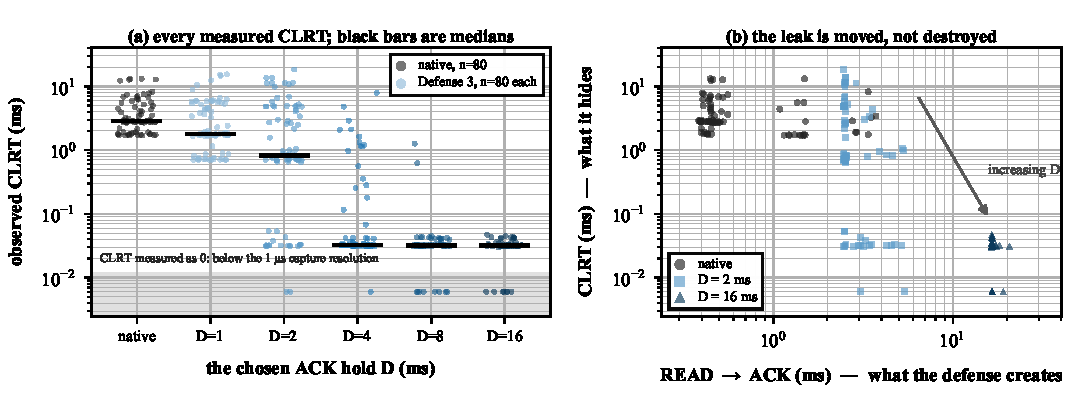
\includegraphics[width=7.16in]{figures/out/fig7_scatter.pdf}}
\caption{\textbf{(a)} Every measured CLRT, one point per transaction, 80 per arm, on a
logarithmic axis; black bars are medians and points are jittered horizontally only. The
native cloud spans \num{1.7}--\num{13.2} ms; by $D=16$ ms the entire cloud has collapsed onto
the \num{32}\,$\mu$s release tail. Points in the grey band were measured as exactly zero, i.e.
below the 1\,$\mu$s resolution of the capture. \textbf{(b)} The same data plotted as the two
observables against each other. The native cloud sits at the left, spread vertically ---
the vertical spread \emph{is} the fingerprint. As $D$ grows the cloud moves right and
flattens: the spread leaves the CLRT axis and appears on the READ$\to$ACK axis. Nothing is
destroyed; it is moved. Source: \code{figures/src/fig7\_scatter.py}.}
\label{fig:scatter}
\end{figure}

\begin{figure}[t]
\centering
\makebox[\textwidth][c]{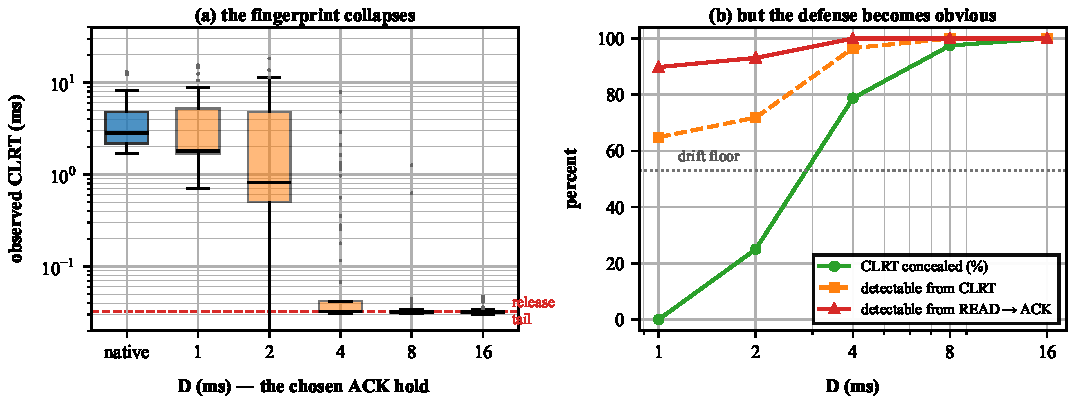
\includegraphics[width=7.16in]{figures/out/fig1_dsweep.pdf}}
\caption{The central result, 480 transactions against the real relay. \textbf{(a)} The
observed CLRT distribution per arm. The whole distribution collapses onto the
\num{32}\,$\mu$s release tail --- the dashed line --- as $D$ grows past the relay's own
response time. \textbf{(b)} The same sweep read two ways: the percentage of transactions
whose CLRT is concealed (green), and how well an adversary separates protected from
unprotected traffic using the CLRT (orange) or using READ$\to$ACK (red). The dotted line is
the native-versus-native drift floor, 53\,\%, which is what ``no information'' looks like in
this session. \textbf{Concealment and detectability rise together, and detection is already
near-perfect where concealment is only partial.}
Source: \code{figures/src/fig1\_dsweep.py}.}
\label{fig:dsweep}
\end{figure}

\begin{keybox}
\textbf{Is the CLRT concealed? Yes.} At $D=16$ ms the CLRT's standard deviation falls from
\num{2.854} ms to \num{0.012} ms --- a factor of about \textbf{240} --- and all 80
transactions land on the same \num{32}\,$\mu$s release tail, with a maximum of \num{0.047}
ms. The feature that was the fingerprint is flattened to a constant. The objective the
threat model sets is met.
\end{keybox}

\subsection{The mechanism held up over 480 transactions}

Per-arm counter totals, identical for every armed arm:

\begin{center}
\begin{tabular}{lrl}
\toprule
\textbf{measurement} & \textbf{value} & \textbf{meaning} \\
\midrule
tokens admitted & \textbf{\num{5 120} $=64\times80$} & exactly $K$ per transaction, every transaction \\
transactions armed & 80 & one per poll \\
tokens ending on the deadline & \textbf{\num{5 120}} & every token, the intended path \\
stale terminations & \textbf{0} & no token ever lost track of its transaction \\
budget expiries / fail-open & \textbf{0} & the safety net was never needed \\
admission drops & \textbf{0} & no token arrived to find no transaction \\
concurrent-transaction refusals & \textbf{0} & every transaction ended before the next began \\
duplicate suppressions & \textbf{0} & the relay retransmitted zero times in 480 \\
queue drops & \textbf{0} & nothing was lost \\
\bottomrule
\end{tabular}
\end{center}

And both state-machine exits partitioned exactly, 400 times:

\begin{center}
\begin{tabular}{lcccc}
\toprule
\textbf{arm} & \textbf{response in window} & \textbf{arrived after}
& \textbf{ended by the ACK} & \textbf{ended by the response} \\
\midrule
d1  & 0  & 80 & \textbf{80} & 0  \\
d2  & 18 & 62 & 62 & 18 \\
d4  & 62 & 18 & 18 & 62 \\
d8  & 78 & 2  & 2  & 78 \\
d16 & 79 & 1  & 1  & 79 \\
\bottomrule
\end{tabular}
\end{center}

The two columns always sum to 80, and ``ended by the ACK'' always equals ``arrived after''.
As $D$ grows past the relay's own response time, transactions migrate from one exit to the
other. This is the state-machine repair sweeping across its own boundary on real traffic,
400 times, with no exceptions --- the strongest evidence in this report that the state
machine is right.

\subsection{The second analysis, which changes how the first should be read}

The table above scores \emph{one} number. A real eavesdropper sees every timing the exchange
produces --- and Defense 3 \textbf{creates} one: READ$\to$ACK becomes $D+\num{0.51}$ ms.

Drift floors, native versus native, are at chance for all three features: READ$\to$ACK
\num{0.514}, CLRT \num{0.530}, READ$\to$RESPONSE \num{0.503}.

\begin{center}
\begin{tabular}{lcccc}
\toprule
\textbf{arm} & \textbf{$D$} & \textbf{READ$\to$ACK} & \textbf{CLRT}
& \textbf{READ$\to$RESPONSE (the total)} \\
\midrule
d1 \emph{null} & 1  & \textbf{\num{0.898}} & \num{0.649} & \num{0.542} \\
d2             & 2  & \textbf{\num{0.931}} & \num{0.719} & \num{0.578} \\
d4             & 4  & \textbf{\num{1.000}} & \num{0.966} & \num{0.669} \\
d8             & 8  & \textbf{\num{1.000}} & \num{1.000} & \num{0.925} \\
d16            & 16 & \textbf{\num{1.000}} & \num{1.000} & \num{1.000} \\
\bottomrule
\end{tabular}
\end{center}

\begin{figure}[t]
\centering

\includegraphics[width=4.35in]{figures/out/report/fig3_observer.pdf}
\caption{Separability from native for each of the three timings an observer can measure, at
every $D$. Bars start at \num{0.50}, which is chance. \textbf{READ$\to$ACK --- the feature
the defense creates --- beats the CLRT at every single $D$}, and the total
READ$\to$RESPONSE is the \emph{least} separable, because while $D$ is below the native CLRT
the defense conserves the total and merely moves time from one term into the other. A bar at
the dotted drift floor would mean no information at all.
Source: \code{figures/src/fig3\_observer.py}.}
\label{fig:observer}
\end{figure}

And a classifier that is \emph{not} fitted on the data it is scored on --- a single threshold
chosen from rounds 1--2 and tested on rounds 3--4, with balanced accuracy so class sizes
cannot flatter it:

\begin{center}
\begin{tabular}{lccc}
\toprule
\textbf{arm} & \textbf{$D$} & \textbf{threshold} & \textbf{balanced accuracy, held out} \\
\midrule
d1 \emph{null} & 1  & \num{0.985} ms & \textbf{\num{0.863}} \\
d2             & 2  & \num{1.495} ms & \textbf{\num{0.950}} \\
d4             & 4  & \num{2.485} ms & \textbf{\num{0.963}} \\
d8             & 8  & \num{4.490} ms & \textbf{\num{1.000}} \\
d16            & 16 & \num{8.485} ms & \textbf{\num{1.000}} \\
\bottomrule
\end{tabular}
\end{center}

Three things follow.

\textbf{The CLRT number was the flattering one.} READ$\to$ACK beats it at every $D$, and the
gap is widest exactly where the defense looked best: at $D=2$ ms the CLRT is only partly
concealed (20/80, separability \num{0.719}) while one threshold on READ$\to$ACK already gets
\num{0.950} on data it never saw.

\textbf{Detectability exceeds the concealment it buys, at every $D$.} Even at $D=1$ ms ---
the null control that conceals \emph{nothing} --- a held-out classifier reaches \num{0.863}.
There is no setting in this sweep at which Defense 3 is harder to detect than the
information it removes.

\textbf{The reason is now measured, not argued.} READ$\to$RESPONSE, the \emph{total}, is the
\textbf{least} separable feature: \num{0.542} at $D=1$ against a \num{0.503} floor ---
essentially unchanged. While $D$ is below the native CLRT, Defense 3 approximately
\textbf{conserves the total} and merely \textbf{redistributes} time out of the CLRT and into
READ$\to$ACK:
\begin{equation}
a + c
\;\;\xrightarrow{\ \text{Defense 3, } D<c\ }\;\;
\underbrace{(a+D)}_{\text{observable 1}} + \underbrace{(c-D)}_{\text{observable 2}}
\;=\; a+c .
\label{eq:conserve}
\end{equation}
That is what ``the leak is relocated, not destroyed'' means, quantitatively: the observable
that survives is the sum, and the leak is the redistribution. Only when $D$ dominates the
total ($D=16$) does the sum separate too --- and by then everything separates at
\num{1.000}.

\subsection{What survives, precisely}

READ$\to$ACK after the hold is $D$ plus the relay's own acknowledgement latency. Since $D$
is our own parameter, and therefore known to anyone who measures a few transactions,
subtract it:

\begin{center}
\begin{tabular}{lrrrr}
\toprule
\textbf{arm} & \textbf{R$\to$A med.} & \textbf{R$\to$A sd} & \textbf{med. $-D$}
& \textbf{sep. of (R$\to$A $-\,D$) vs native} \\
\midrule
native & \num{0.453}  & \textbf{\num{0.825}} & ---          & (floor \textbf{\num{0.514}}) \\
d1     & \num{1.514}  & \num{0.798} & \num{0.514} & \num{0.690} \\
d2     & \num{2.515}  & \num{0.771} & \num{0.515} & \num{0.702} \\
d4     & \num{4.508}  & \num{0.680} & \num{0.508} & \num{0.679} \\
d8     & \num{8.519}  & \num{0.347} & \num{0.519} & \num{0.683} \\
d16    & \num{16.509} & \num{0.588} & \num{0.509} & \num{0.660} \\
\bottomrule
\end{tabular}
\end{center}

\textbf{The spread is essentially untouched} --- \num{0.35} to \num{0.80} ms after the
defense against \num{0.825} ms before. The hold \emph{translates} the acknowledgement-latency
distribution by $D$; it does not compress it. Subtracting $D$ recovers something only
\num{0.66}--\num{0.70} separable from native against a \num{0.514} floor: not a perfect
reconstruction, thanks to a systematic $+\num{0.06}$ ms the switch adds, but far closer to
native than the raw READ$\to$ACK at \num{1.000}.

So the relay's own acknowledgement latency --- a \emph{different} device property from CLRT
--- passes through this defense with its shape intact.

%======================================================================
\section{What may and may not be claimed}
\label{sec:claims}

\subsection{Established}

\begin{enumerate}[leftmargin=1.5em,itemsep=0.25em]
\item \textbf{The mechanism works on real hardware.} 480 of 480 transactions, exactly 64
  tokens each, all terminating on the deadline, zero fail-open, zero drops, ordering correct
  480 of 480, hold accurate to $-\num{168}$ ns on the physical relay.
\item \textbf{The hold is governed by $D$ and nothing else.} READ$\to$ACK $=D+\num{0.51}$ ms
  at five values of $D$ spanning 1 to 16 ms.
\item \textbf{CLRT concealment.} Standard deviation \num{2.854} $\to$ \num{0.012} ms, a
  factor of ${\approx}\,240$; 80 of 80 transactions flattened onto a \num{32}\,$\mu$s
  constant at $D=16$ ms.
\item \textbf{The state machine is correct across its whole domain.} \num{2 256} exhaustive
  assertions, mutation-checked, plus 400 physical transactions in which the two exits
  partitioned perfectly.
\item \textbf{Graceful degradation.} When $D$ is smaller than the CLRT the output is $c-D$,
  not the untouched CLRT --- a partial rather than a cliff-edge failure.
\item \textbf{Non-transaction traffic is not disturbed.} Real relay keepalives were rejected
  and forwarded, on real traffic, three for three.
\end{enumerate}

\subsection{Not established, and why}

\begin{enumerate}[leftmargin=1.5em,itemsep=0.3em]
\item \textbf{Device anonymity.} Concealing CLRT is not the same as making the device
  unidentifiable, and this report does \emph{not} demonstrate the latter. The relay's own
  acknowledgement latency survives with its spread intact. Worse, the question cannot be
  answered with this data at all: \textbf{there is no confusion set}. The other devices in
  the corpus are combined-ACK, separable on packet count alone. \textbf{One relay cannot
  answer a discrimination question}, however many transactions are run against it. Settling
  it needs a second \emph{separate-ACK} device measured under the same $D$.
\item \textbf{``Better than Defense 2''.} No iso-latency Defense 2 arm was run --- it needs a
  different switch program. And it must be matched on \emph{added latency}, not on the
  parameter: comparing $D\le3$ ms against $G=25$ ms is uninterpretable in both directions.
  The numerical target is now known, since Defense 3's added latency is ${\approx}\,D$.
\item \textbf{Undetectability.} The opposite is established. Detection is perfect at
  $D\ge8$ ms and \num{0.863} even at the null control.
\item \textbf{A steady-state CLRT for the SEL-751.} One relay, one session, one 200 ms poll
  rate. The relay has at least two timing regimes --- a connection-cold first poll and a
  steady state --- so the \num{2.828} ms median here is this session's distribution, not the
  device's.
\item \textbf{$K=64$ is minimal.} It is sufficient, and it is what was measured. No smaller
  value was tested.
\item \textbf{Concurrency.} One active protected transaction at a time. This is the
  \emph{measured capacity} of the mechanism --- a hold consumes roughly 24 of the
  25\,Gbit/s internal loopback --- not a prototype simplification that a later version
  removes.
\item \textbf{Segmentation.} Every response in the corpus and in every test was a single
  segment. Multi-segment responses are detected and forwarded unprotected, not handled.
\end{enumerate}

\subsection{Open work, and what each item blocks}

\begin{center}\small
\begin{tabular}{@{}>{\raggedright\arraybackslash}p{0.03\textwidth}>{\raggedright\arraybackslash}p{0.225\textwidth}>{\raggedright\arraybackslash}p{0.235\textwidth}>{\raggedright\arraybackslash}p{0.355\textwidth}@{}}
\toprule
\textbf{\#} & \textbf{open item} & \textbf{what it blocks} & \textbf{why it is not done} \\
\midrule
1 & iso-latency Defense 2 arm & any Defense 2 vs Defense 3 statement, either direction
  & needs a different switch program loaded; $G$ must match \emph{added latency}, so
    $G\approx D+\text{native CLRT}$ \\
2 & a $D$ calibrated on one campaign and tested on another & selecting an operating point
  & the governing constraints forbid fitting and testing $D$ on the same campaign; the sweep
    here does not fit, so nothing is violated --- but nothing is selected either \\
3 & a second separate-ACK device & the device-anonymity question in any form
  & not available; a corpus limitation, not a schedule one \\
4 & safety tests as a named stage & nothing already covered
  & fail-open, keepalive, concurrent, stale and duplicate cases are all exercised above;
    superseded in substance, never in form \\
5 & the $D=40$ ms clamp boundary & nothing in the claims
  & an input-validation edge, never exercised \\
6 & multi-segment responses & nothing claimed
  & every response in the corpus was a single segment, so the path has never been taken \\
7 & rollback to Defense 2 & nothing; it is deliberate
  & the switch is intentionally left running Defense 3 with the reservoir armed \\
\bottomrule
\end{tabular}
\end{center}

\subsection{Stated head-on rather than buried}

At the values of $D$ that actually conceal, \textbf{the output is physically implausible}. A
device that took \num{16.5} ms to acknowledge a 20-byte read and then answered
\num{32}\,$\mu$s later, every single time, resembles no real relay: generating an
acknowledgement is cheap and computing an answer is expensive, so the defense
\textbf{inverts the natural ordering of costs}. Defense 2's output stays inside the space of
plausible device behaviour; Defense 3's, at the $D$ that conceals, leaves it.

\textbf{Safety.} Every physical transaction in this report was a \emph{read}. No SELECT, no
OPERATE, no DIRECT OPERATE, no configuration write, no setting change and no cold restart
was ever sent to the relay --- not once in 480 transactions plus the smoke tests. The
defense never modifies a byte of any packet; it only changes \emph{when} packets leave.

%======================================================================
\section{How to reproduce everything}

\subsection{Software only, no hardware}

\begin{center}\small
\begin{tabular}{@{}>{\raggedright\arraybackslash}p{0.50\textwidth}>{\raggedright\arraybackslash}p{0.36\textwidth}@{}}
\toprule
\textbf{command} (from \code{defense3/}) & \textbf{what it checks} \\
\midrule
\code{python3 analysis/test\_tag\_domain.py} & \num{2 256} assertions; exit 0 \\
\code{python3 analysis/analyze\_defense3.py -{}-self-test} & 17 negative controls \\
\code{python3 analysis/analyze\_gate34.py -{}-self-test} & 20 controls \\
\code{python3 analysis/analyze\_check2.py -{}-self-test} & 6 controls \\
\code{python3 analysis/analyze\_dsweep.py} \newline
  \code{\quad evidence/physical/dsweep\_blocks.jsonl /tmp/a.json}
  & regenerates the sweep tables \\
\code{python3 analysis/analyze\_observer.py} \newline
  \code{\quad evidence/physical/dsweep\_blocks.jsonl /tmp/b.json}
  & regenerates the observer tables \\
\bottomrule
\end{tabular}
\end{center}

The last two regenerate every table in \S\ref{sec:campaign} from the raw per-transaction
data.

\subsection{Compiling}

\begin{center}\small
\begin{minipage}{0.86\textwidth}
\code{bf-p4c -{}-target tofino -{}-arch tna -g \textbackslash}\\
\code{\quad\ [-DD3\_SYNTH\_EVENTS | -DD3\_LIVE\_FULL\_TELEMETRY] \textbackslash}\\
\code{\quad\ -o <outdir> \textbackslash}\\
\code{\quad\ p4/case\_a\_defense3\_fixed\_ack\_delay.p4}\\
\code{python3 analysis/assert\_salu\_asm.py <outdir>}\quad\# this MUST pass
\end{minipage}
\end{center}

Three configurations: no flag is the core live build (9/12 stages);
\code{D3\_LIVE\_FULL\_TELEMETRY} is live plus the two internal timestamps (10/12);
\code{D3\_SYNTH\_EVENTS} is the synthetic test build (9/12). Never compile the synthetic flag
for live use --- it relaxes an acceptance conjunct so that generated packets can reach the
real hold path.

\subsection{The figures}

Every figure in this document is regenerated by one script under \code{figures/src/}, run
with \code{\$RESEARCH\_PYTHON}:

\begin{center}\small
\begin{tabular}{@{}ll@{}}
\toprule
\textbf{script} & \textbf{figure} \\
\midrule
\code{fig1\_dsweep.py}       & Fig.~\ref{fig:dsweep} --- the $D$-sweep result \\
\code{fig2\_mechanism.py}    & Fig.~\ref{fig:mechanism} --- construction and hold decomposition \\
\code{fig3\_observer.py}     & Fig.~\ref{fig:observer} --- per-feature separability \\
\code{fig4\_timelines.py}    & Fig.~\ref{fig:timelines} --- the four defenses on one axis \\
\code{fig5\_statemachine.py} & Fig.~\ref{fig:fsm} --- the transaction state machine \\
\code{fig6\_trigger.py}      & Fig.~\ref{fig:trigger} --- the trigger chain and its margin \\
\code{fig7\_scatter.py}      & Fig.~\ref{fig:scatter} --- every raw CLRT, native and defended \\
\code{fig8\_topology.py}     & Fig.~\ref{fig:topology} --- the physical setup \\
\bottomrule
\end{tabular}
\end{center}

Each script reads \code{evidence/physical/dsweep\_blocks.jsonl} or the measured constants
quoted here, recomputes every number it plots, and prints them, so a figure can be checked
against the tables. Output is vector PDF plus 300 dpi PNG at IEEE column widths
(3.5 in single, 7.16 in double) with 9 pt Times New Roman, so nothing is rescaled on the
page. Palette \code{alessandretti-nature}, one colour per meaning across all eight figures.

The one deviation from the figure conventions: the schematics are drawn in matplotlib rather
than Inkscape. That trades a little typographic polish for the diagrams being
\emph{regenerable from the same scripts as the data panels} --- no manual step between the
measurements and the drawing.

\subsection{On hardware}

Loading displaces whatever is running and needs explicit authorization. The synthetic gates
are \code{./run/run\_defense3.sh -{}-gate2} (one transaction), \code{-{}-gate3} (five
consecutive), \code{-{}-gate4} (the boundary cases) and \code{-{}-check2} (trigger latency,
100 trials). The runner loads nothing itself, asserts the loopback speed before and after,
refuses to start on dirty state, and always restores --- deliberately delegating restoration
to the one existing copy of that code rather than reimplementing it.

The physical campaign is \code{harness/campaign.sh out.jsonl 4 20 0.2} (rounds, polls per
block, gap in seconds), with \code{harness/setarm.py} on the switch (sets $D$, arms the
reservoir, clears per-transaction state) and \code{harness/block.py} on the master
(captures, polls, parses the capture into per-transaction rows).

%======================================================================
\section{Every mistake made, and what it cost}

Recorded because the pattern is more useful than the individual bugs: \textbf{in this
project, tests and criteria were wrong about as often as the code was.}

\begin{center}\small
\begin{longtable}{@{}>{\raggedright\arraybackslash}p{0.03\textwidth}>{\raggedright\arraybackslash}p{0.355\textwidth}>{\raggedright\arraybackslash}p{0.255\textwidth}>{\raggedright\arraybackslash}p{0.255\textwidth}@{}}
\toprule
\textbf{\#} & \textbf{mistake} & \textbf{how it was found} & \textbf{cost} \\
\midrule
\endhead
1 & Graded the design against a broader objective than the threat model sets, and concluded
  ``do not build'' & corrected by the project lead & one wrong verdict, reversed \\
2 & Quoted $D=12$ ms as reaching a 99th percentile of \num{12.607} ms & caught in review
  & corrected to 13 \\
3 & Pooled a connection-cold poll into a ``steady-state'' sample & a review pass
  & $D$ for a full clamp was 13 ms, not 22 \\
4 & Large constant in stateful hardware; the write silently never committed
  & reading the compiled assembly, after two wrong theories & the whole of \S\ref{sec:traps} \\
5 & Then claimed the \emph{cause} was proven from the assembly
  & a 13-constant probe showed identical output for all $K$ & claim narrowed to an inference \\
6 & Moving the idle marker collided it with a different sentinel; both transaction exits
  became no-ops & an audit, before it ever ran & would have broken every second transaction \\
7 & Counted the defense's own mirrored copy as an off-topology packet & the same audit
  & made a gate requirement unsatisfiable whenever the defense worked \\
8 & Left a stale \code{0xFF} in the scoring code & the same audit & a gate could never pass again \\
9 & Put all synthetic events in one generator run
  & measured \num{1 000 012} ns, reproduced to the nanosecond & discovered the generator run-span law \\
10 & Assumed a pattern-triggered generator can label its packets
  & three roles collapsed into one & forced the two-timer design \\
11 & Set the token increment in the wrong branch of the classifier
  & 16 admitted then 48 dropped: $\code{0xC0}+16=\code{0xD0}$ leaves the valid range exactly
    at token 17 & one silicon run \\
12 & Clean-state criterion demanded zeros the architecture never promised
  & Gate 3 stopped at transaction 2 & replaced with a \emph{stricter} rule \\
13 & Sign test written unsigned; always false & the assembly assertion, which now blocks it
  & \S\ref{sec:traps} \\
14 & Duplicate-response rubric never tested ordering & added a timestamp and looked
  & the duplicate was overtaking the held ACK by \num{1.0014} ms \\
15 & That new timestamp also fired on the \emph{dropped} copy
  & the gate failed against a packet that departed nowhere & one analysis pass \\
16 & Scored a boundary case with the normal-transaction rubric, which forbids the bypass the
  case exists to produce & the gate failed on its own purpose & one analysis pass \\
17 & No live arming step, so the first physical run had an empty hold queue
  & the registers said \code{app\_enable = false} & one physical run, stopped and preserved \\
18 & Per-block counter zeroing failed silently; cumulative snapshots were summed
  & the totals were absurd (307 arms for 80 polls)
  & one arm's counters unusable; recovered by differencing \\
19 & Reported concealment on one feature & asked what an eavesdropper actually gets
  & \S\ref{sec:campaign} --- the headline result changed \\
\bottomrule
\end{longtable}
\end{center}

The two that generalise:

\begin{keybox}
\textbf{A test that cannot fail proves nothing.} Every checker in this directory has negative
controls, and every one of them was mutation-checked --- because four of the nineteen
mistakes above were mistakes in the \emph{checker}, not in the mechanism.

\smallskip
\textbf{A silent success is not a success.} Two of the four hardware traps compiled cleanly
and produced no error at run time; one of them produced a \emph{counter} saying the opposite
of the truth. On this hardware, ``it compiled and nothing complained'' carries almost no
information.
\end{keybox}

%======================================================================
\section{Summary}

Defense 3 holds a DNP3 outstation's TCP acknowledgement to a predetermined instant
$t_{\mathrm{ACK}}+D$, released independently of the response, using nothing but a crowd of
recirculating dummy packets and the switch's own strict-priority scheduler. It is
implemented entirely in the data plane of an Intel Tofino-1, generates its own blocker
tokens on chip, touches no packet byte, and requires no cooperation from the relay.

It does what it was built to do. The CLRT --- the cross-layer timing fingerprint that prior
work uses to identify equipment --- collapses from a \num{2.854} ms standard deviation to
\num{0.012} ms, and at $D=16$ ms every one of 80 transactions lands on the same
\num{32}\,$\mu$s constant. The mechanism ran 480 physical transactions against a real
SEL-751 with zero fail-open events, zero dropped packets and the
acknowledgement-before-response ordering correct every single time.

And it is not a finished defense. It creates a new timing feature, READ$\to$ACK, which is
more separable from native traffic than the CLRT it removes --- at \emph{every} value of
$D$, including the null control that conceals nothing. Equation~\eqref{eq:conserve} says why:
while $D$ is below the native CLRT the total is conserved and the defense merely
redistributes it. At the $D$ that conceals fully, the output does not resemble any physical
device. Both facts were measured here, not argued, and both are stated in
\S\ref{sec:claims} rather than left for a reviewer to find.

The next experiment is named and its target value is known: an iso-latency Defense 2 arm at
$G\approx D+\text{native CLRT}$, which is the only way to say whether holding the
acknowledgement or holding the response is the better trade.

\end{document}
